
\section{Background} \label{sec:background}

We assume a background on LLMs, including their transformer-based architecture (\Cref{app:llm-transformer}), in-context learning (\Cref{sec:icl-performance}), and reinforcement learning (full preliminaries are provided in \Cref{app:technicality}). We briefly review the literature on mnemonic devices for vocabulary learning and the use of LLMs in linguistic tasks.

\subsection{Mnemonic devices for vocabulary learning} \label{sec:mnemonic-review}

% TODO: Add a figure for what good mnemonics means. Here is a placeholder
% \begin{figure*}[htb]
%   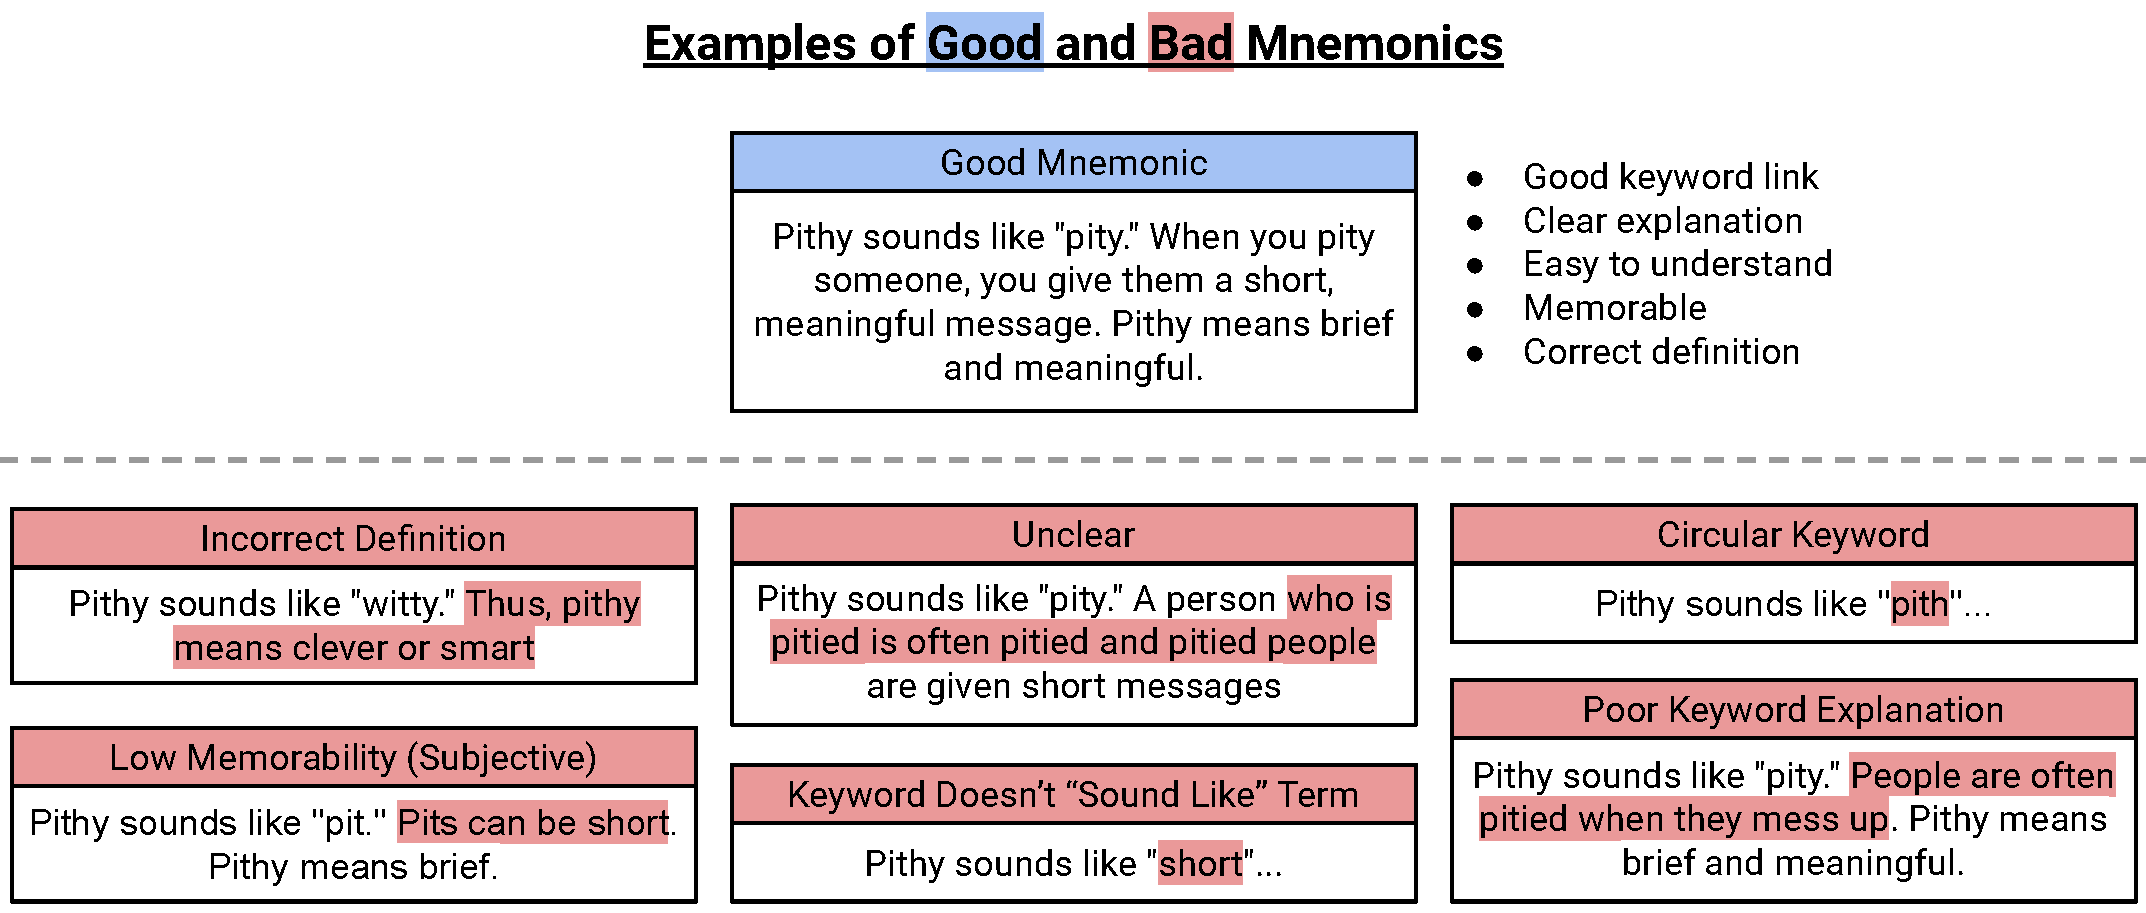
\includegraphics[width=\linewidth]{figures/good_bad_mnemonics.pdf}
%   \caption{Non-exhausitive list of characteristics of a good mnemonic, inferred from \citetext{\citealp{BalepurSMART2024}; \citealp{CamposUSING2011}; \citealp{luExplorationMnemonicsESL2015}; \citealp{SariogluUSE2024}}.}
%   \label{fig:good-bad-mnemonics}
% \end{figure*}

% Define custom colors


% Define custom box styles
\tcbset{
    goodbox/.style={
        colback=goodlight,
        colframe=goodgreen,
        fonttitle=\bfseries\color{white},
        coltitle=white,
        colbacktitle=goodgreen,
        enhanced,
        attach boxed title to top center={yshift=-1mm},
        boxed title style={sharp corners},
        top=2mm,
    },
    badbox/.style={
        colback=badlight,
        colframe=badred,
        fonttitle=\bfseries\color{white},
        coltitle=white,
        colbacktitle=badred,
        enhanced,
        attach boxed title to top center={yshift=-1mm},
        boxed title style={sharp corners},
        top=2mm,
    }
}

% Start the figure environment
\begin{figure*}[htb]
\centering
\footnotesize
% First row - Good mnemonic + characteristics
\begin{minipage}{0.66\textwidth}
    \begin{tcolorbox}[goodbox, title=Good Mnemonic]
        \textcolor{red}{\textbf{preposterous}}: \textcolor{goodgreen}{comes from pre- ("before") + post ("after") + -ous}, meaning reversed or absurd. \textcolor{orange}{An event cannot happen both pre- (before) and post- (after) to us, it is prespoterous!}
    \end{tcolorbox}
\end{minipage}
\hspace{0.5em}
\begin{minipage}{0.3\textwidth}
    \begin{itemize}[leftmargin=*, nosep]
        \item \vocab is used correctly in \mnem
        \item Clear \assoc linking \vocab and \mnem
        \item Strong \assoc
        \item \mnem uses similar or lower vocabulary than \vocab
        \item \mnem is memorable
    \end{itemize}
\end{minipage}

\vspace{0.3cm}

% Second row - 3 bad mnemonics
\begin{minipage}{0.33\textwidth}
    \begin{tcolorbox}[badbox, title=Incorrect Definition]
        Preposterous means very important or significant.
    \end{tcolorbox}
\end{minipage}%
\begin{minipage}{0.33\textwidth}
    \begin{tcolorbox}[badbox, title=Circular Association]
        Preposterous sounds like preposterous.
    \end{tcolorbox}
\end{minipage}%
\begin{minipage}{0.33\textwidth}
    \begin{tcolorbox}[badbox, title=Weak Association]
        Preposterous sounds like prosperous. Preposterous people usually make prosperous business decisions.
    \end{tcolorbox}
\end{minipage}

\vspace{0.3cm}

% Third row - 3 more bad mnemonics
\begin{minipage}{0.33\textwidth}
    \begin{tcolorbox}[badbox, title=Difficult Vocabulary]
        Preposterous means ludicrously implausible or contrary to conventional hierarchies of logical induction.
    \end{tcolorbox}
\end{minipage}%
\begin{minipage}{0.33\textwidth}
    \begin{tcolorbox}[badbox, title=Too Abstract]
        Preposterous describes logical fallacies where the premise negates itself through temporal displacement.
    \end{tcolorbox}
\end{minipage}%
\begin{minipage}{0.33\textwidth}
    \begin{tcolorbox}[badbox, title=Offensive Content]
        Preposterous contains "post" which reminds me of [inappropriate culturally-specific reference].
    \end{tcolorbox}
\end{minipage}

\caption{Characteristics of good mnemonics, and examples of bad mnemonics. We propose VAM/VEM model, where a good mnemonic must have three components: \vocabulary (\vocab), \association (\assoc) (or explanation ($e$)), and \mnemonic (\mnem), with characteristics listed above. These characteristics are also available in list (\Cref{app:mnemonic-characteristics})}
\label{fig:good-bad-mnemonics}
\end{figure*}



\begin{table*}[htb]
\centering
\caption{Examples of feature categories for English words.}
\label{tab:linguistic-features}
\begin{tabularx}{\textwidth}{l >{\raggedright\arraybackslash}X >{\raggedright\arraybackslash}X}
\toprule
\textbf{feature} & \textbf{description} & \textbf{example} \\
\midrule
\textbf{phonetics} & sound patterns & \emph{apparent} sounds like “a bare Asian.” \\
\addlinespace
\textbf{orthography} & written/spelling patterns & \emph{abet} looks like “a + bet.” \\
\addlinespace
\textbf{morphology} & modern English forms, including free and bound morphemes & \emph{aggrandize} = a + grand + –ize, to mean to make grander. \\
\addlinespace
\textbf{etymology} & origin and history & \emph{adumbrate} comes from Latin ad- (to, on) + umbra (shade) + ate, to mean foreshadow or outline. \\
\addlinespace
\textbf{semantics} & meaning and semantic relationships & \emph{confound} has similar meaning and history with 'confuse'. \\
\bottomrule
\end{tabularx}
\end{table*}
\subsection{LLMs: linguistic competence and creativity} \label{sec:llm-linguistic-competence}
